\documentclass[tikz,border=8pt]{standalone}
\usepackage{ctex}
\usepackage{amsmath,amssymb}
\usetikzlibrary{arrows.meta,calc,angles,quotes,patterns,positioning,decorations.pathmorphing}
\definecolor{ink}{RGB}{30,43,58}
\definecolor{blue}{RGB}{38,92,168}
\definecolor{orange}{RGB}{220,112,24}
\definecolor{green}{RGB}{38,139,93}
\definecolor{red}{RGB}{192,53,53}
\tikzset{
 line cap=round,line join=round,
 body/.style={draw=ink,very thick},
 axis/.style={-{Latex[length=2.5mm]},draw=ink,very thick},
 vec/.style={-{Latex[length=2.5mm]},draw=blue,very thick},
 force/.style={-{Latex[length=2.5mm]},draw=red,very thick},
 guide/.style={draw=ink!48,dashed},
 dim/.style={{Latex[length=2mm]}-{Latex[length=2mm]},draw=ink!70}
}

\usetikzlibrary{decorations.pathmorphing}
\tikzset{mass/.style={circle,draw,fill=white,minimum size=7mm},curve/.style={very thick,blue},rope/.style={very thick,blue},ray/.style={very thick,blue,-{Latex}},impulse/.style={very thick,orange,-{Latex}},current/.style={very thick,orange,-{Latex}},resistor/.style={thick,decorate,decoration={zigzag,segment length=3mm,amplitude=1mm}}}
\begin{document}
% 1 question-01
\begin{tikzpicture}[x=1cm,y=1cm,font=\small]

\draw[guide] (-.3,0)--(8,0);
\draw[body,fill=blue!12] (0,0) rectangle (2,1);
\draw[body,fill=orange!12] (4,0) rectangle (6,1);
\node at (1,.5) {后车};\node at (5,.5) {前车};
\draw[dim] (2,-.45)--(4,-.45) node[midway,below] {$d$};
\fill[red] (2,.05) circle(2pt);\fill[red] (4,.05) circle(2pt);
\node[anchor=north] at (2,-1) {后车头};\node[anchor=north] at (4,-1) {前车尾};
\draw[vec] (4,1.4)--(6,1.4) node[midway,above] {$v_F$};
\draw[vec] (0,1.4)--(2,1.4) node[midway,above] {$v_R$};
\node[align=left,anchor=west] at (6.5,.6) {$d_0=2\,\mathrm m$\\启动门槛 $d_s=7\,\mathrm m$};

\end{tikzpicture}

% 2 solution-01
\begin{tikzpicture}[x=1cm,y=1cm,font=\small]

\begin{scope}
\draw[axis] (0,0)--(5.6,0) node[right] {$t$};\draw[axis] (0,0)--(0,3) node[above] {$v$};
\fill[blue!12] (0,0)--(3,2.4)--(4,2.4)--(1,0)--cycle;
\draw[blue,very thick] (0,0)--(3,2.4)--(5,2.4);
\draw[orange,very thick] (1,0)--(4,2.4)--(5,2.4);
\node[blue] at (1.1,2.6) {前车};\node[orange] at (4.1,1.3) {后车};
\draw[dim] (0,-.4)--(1,-.4) node[midway,below] {$\Delta$};
\node[align=center] at (2.5,-1.2) {启动：$\Delta d=v\Delta$};
\end{scope}
\begin{scope}[xshift=7cm]
\draw[axis] (0,0)--(5.6,0) node[right] {$t$};\draw[axis] (0,0)--(0,3) node[above] {$v$};
\fill[orange!13] (0,2.4)--(1,2.4)--(4,0)--(3,0)--cycle;
\draw[blue,very thick] (0,2.4)--(3,0)--(5,0);
\draw[orange,very thick] (0,2.4)--(1,2.4)--(4,0)--(5,0);
\node[blue] at (1,.7) {前车};\node[orange] at (3.6,1.5) {后车};
\draw[dim] (0,-.4)--(1,-.4) node[midway,below] {$\tau$};
\node[align=center] at (2.5,-1.2) {制动：$\Delta d=-v\tau$};
\end{scope}

\end{tikzpicture}

% 3 question-02
\begin{tikzpicture}[x=1cm,y=1cm,font=\small]

\draw[body] (0,-1)--(0,1.8);\draw[body] (4,-1)--(4,1.8);
\draw[guide] (0,0)--(4,0);
\draw[blue,very thick,domain=0:4,samples=100] plot(\x,{.7*sin(135*\x)});
\draw[dim] (0,-1.35)--(4,-1.35) node[midway,below] {$L=n\lambda_n/2$};
\node at (2,2.1) {$n=3$ 驻波示例};
\begin{scope}[xshift=8cm]
\draw[body] (0,0) circle(1.8);\draw[blue,very thick] (90:1.8)--(210:1.8)--(330:1.8)--cycle;
\draw[orange,very thick,dashed] (45:1.8)--(135:1.8)--(225:1.8)--(315:1.8)--cycle;
\draw[dim] (0,0)--(25:1.8) node[midway,below] {$R$};
\node at (0,-2.5) {闭合轨道的传播相位条件};
\end{scope}

\end{tikzpicture}

% 4 solution-02
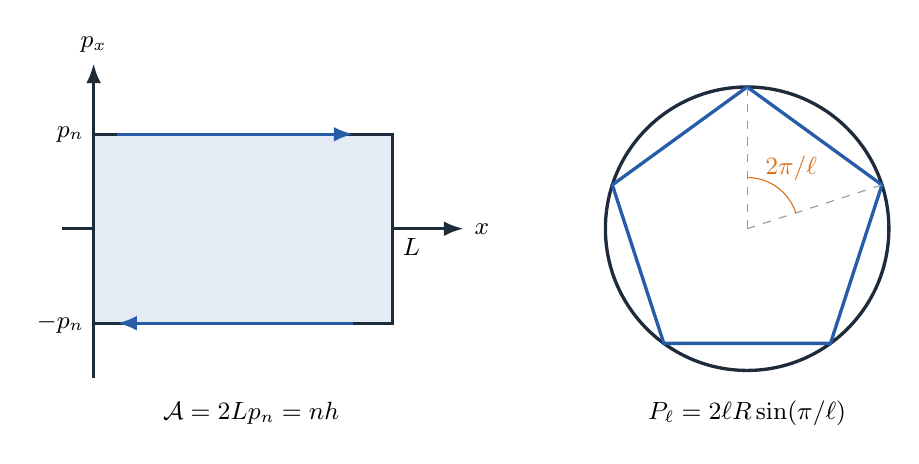
\begin{tikzpicture}[x=1cm,y=1cm,font=\small]

\draw[axis] (-.4,0)--(4.7,0) node[right] {$x$};\draw[axis] (0,-1.9)--(0,2.1) node[above] {$p_x$};
\fill[blue!12] (0,-1.2) rectangle (3.8,1.2);
\draw[body] (0,-1.2) rectangle (3.8,1.2);
\draw[vec] (.3,1.2)--(3.3,1.2);\draw[vec] (3.3,-1.2)--(.3,-1.2);
\node[left] at (0,1.2) {$p_n$};\node[left] at (0,-1.2) {$-p_n$};\node[below right] at (3.8,0) {$L$};
\node at (2,-2.35) {$\mathcal A=2Lp_n=nh$};
\begin{scope}[xshift=8.3cm]
\draw[body] (0,0) circle(1.8);\draw[blue,very thick] (90:1.8)--(18:1.8)--(-54:1.8)--(-126:1.8)--(162:1.8)--cycle;
\draw[guide] (0,0)--(90:1.8);\draw[guide] (0,0)--(18:1.8);
\draw[orange] (18:.65) arc[start angle=18,end angle=90,radius=.65];
\node[orange] at (54:.95) {$2\pi/\ell$};
\node at (0,-2.35) {$P_\ell=2\ell R\sin(\pi/\ell)$};
\end{scope}

\end{tikzpicture}

% 5 question-03
\begin{tikzpicture}[x=1cm,y=1cm,font=\small]

\draw[body,fill=blue!8] (0,0) circle(2.1);
\draw[guide] (0,0) circle(1.1);
\fill (0,0) circle(2pt) node[below] {$O$};
\draw[dim] (0,0)--(25:2.1) node[midway,below] {$r=ar_0$};
\fill[orange] (25:2.1) circle(3pt);
\draw[vec] (25:2.1)--(25:3.2) node[midway,above] {$\dot r=Hr$};
\node[align=left,anchor=west] at (4,.7) {$M=\dfrac{4\pi}{3}\rho r^3=\mathrm{const}$\\[8pt] $\rho=\rho_0a^{-3}$\\[8pt] 共动球跟踪同一批物质};

\end{tikzpicture}

% 6 solution-03
\begin{tikzpicture}[x=1cm,y=1cm,font=\small]
\draw[axis] (0,0)--(7,0) node[right] {$t/t_0$};\draw[axis] (0,0)--(0,4) node[above] {归一化量};
\draw[very thick,blue] plot coordinates {(1.950000,1.125555) (1.998876,1.144285) (2.047753,1.162864) (2.096629,1.181294) (2.145506,1.199583) (2.194382,1.217733) (2.243258,1.235748) (2.292135,1.253633) (2.341011,1.271392) (2.389888,1.289027) (2.438764,1.306543) (2.487640,1.323942) (2.536517,1.341227) (2.585393,1.358402) (2.634270,1.375468) (2.683146,1.392430) (2.732022,1.409289) (2.780899,1.426047) (2.829775,1.442708) (2.878652,1.459273) (2.927528,1.475744) (2.976404,1.492124) (3.025281,1.508415) (3.074157,1.524618) (3.123034,1.540736) (3.171910,1.556770) (3.220787,1.572721) (3.269663,1.588592) (3.318539,1.604384) (3.367416,1.620099) (3.416292,1.635738) (3.465169,1.651303) (3.514045,1.666794) (3.562921,1.682214) (3.611798,1.697564) (3.660674,1.712844) (3.709551,1.728057) (3.758427,1.743202) (3.807303,1.758283) (3.856180,1.773299) (3.905056,1.788252) (3.953933,1.803142) (4.002809,1.817971) (4.051685,1.832740) (4.100562,1.847450) (4.149438,1.862101) (4.198315,1.876695) (4.247191,1.891233) (4.296067,1.905714) (4.344944,1.920141) (4.393820,1.934514) (4.442697,1.948834) (4.491573,1.963101) (4.540449,1.977317) (4.589326,1.991482) (4.638202,2.005596) (4.687079,2.019661) (4.735955,2.033678) (4.784831,2.047646) (4.833708,2.061567) (4.882584,2.075440) (4.931461,2.089268) (4.980337,2.103050) (5.029213,2.116787) (5.078090,2.130479) (5.126966,2.144128) (5.175843,2.157733) (5.224719,2.171296) (5.273596,2.184816) (5.322472,2.198295) (5.371348,2.211733) (5.420225,2.225129) (5.469101,2.238486) (5.517978,2.251803) (5.566854,2.265080) (5.615730,2.278319) (5.664607,2.291520) (5.713483,2.304682) (5.762360,2.317807) (5.811236,2.330895) (5.860112,2.343947) (5.908989,2.356962) (5.957865,2.369941) (6.006742,2.382885) (6.055618,2.395794) (6.104494,2.408668) (6.153371,2.421507) (6.202247,2.434313) (6.251124,2.447086) (6.300000,2.459824)};
\node[blue,anchor=west] at (7.4,3.2) {$a$};
\draw[very thick,orange] plot coordinates {(1.950000,2.307692) (1.998876,2.251265) (2.047753,2.197531) (2.096629,2.146302) (2.145506,2.097408) (2.194382,2.050691) (2.243258,2.006011) (2.292135,1.963235) (2.341011,1.922246) (2.389888,1.882934) (2.438764,1.845197) (2.487640,1.808943) (2.536517,1.774086) (2.585393,1.740548) (2.634270,1.708253) (2.683146,1.677136) (2.732022,1.647131) (2.780899,1.618182) (2.829775,1.590232) (2.878652,1.563232) (2.927528,1.537133) (2.976404,1.511891) (3.025281,1.487465) (3.074157,1.463816) (3.123034,1.440907) (3.171910,1.418704) (3.220787,1.397174) (3.269663,1.376289) (3.318539,1.356018) (3.367416,1.336336) (3.416292,1.317218) (3.465169,1.298638) (3.514045,1.280576) (3.562921,1.263009) (3.611798,1.245917) (3.660674,1.229282) (3.709551,1.213085) (3.758427,1.197309) (3.807303,1.181939) (3.856180,1.166958) (3.905056,1.152352) (3.953933,1.138107) (4.002809,1.124211) (4.051685,1.110649) (4.100562,1.097411) (4.149438,1.084484) (4.198315,1.071859) (4.247191,1.059524) (4.296067,1.047470) (4.344944,1.035687) (4.393820,1.024166) (4.442697,1.012898) (4.491573,1.001876) (4.540449,0.991091) (4.589326,0.980536) (4.638202,0.970203) (4.687079,0.960086) (4.735955,0.950178) (4.784831,0.940472) (4.833708,0.930962) (4.882584,0.921643) (4.931461,0.912509) (4.980337,0.903553) (5.029213,0.894772) (5.078090,0.886160) (5.126966,0.877712) (5.175843,0.869424) (5.224719,0.861290) (5.273596,0.853308) (5.322472,0.845472) (5.371348,0.837778) (5.420225,0.830224) (5.469101,0.822804) (5.517978,0.815516) (5.566854,0.808356) (5.615730,0.801321) (5.664607,0.794406) (5.713483,0.787611) (5.762360,0.780930) (5.811236,0.774362) (5.860112,0.767903) (5.908989,0.761552) (5.957865,0.755304) (6.006742,0.749158) (6.055618,0.743112) (6.104494,0.737162) (6.153371,0.731306) (6.202247,0.725543) (6.251124,0.719871) (6.300000,0.714286)};
\node[orange,anchor=west] at (7.4,2.55) {$H/H_0$};
\draw[very thick,green] plot coordinates {(1.950000,3.550296) (1.998876,3.378795) (2.047753,3.219428) (2.096629,3.071076) (2.145506,2.932746) (2.194382,2.803556) (2.243258,2.682719) (2.292135,2.569529) (2.341011,2.463354) (2.389888,2.363626) (2.438764,2.269835) (2.487640,2.181517) (2.536517,2.098255) (2.585393,2.019671) (2.634270,1.945420) (2.683146,1.875189) (2.732022,1.808695) (2.780899,1.745675) (2.829775,1.685892) (2.878652,1.629129) (2.927528,1.575185) (2.976404,1.523877) (3.025281,1.475035) (3.074157,1.428504) (3.123034,1.384141) (3.171910,1.341813) (3.220787,1.301397) (3.269663,1.262780) (3.318539,1.225857) (3.367416,1.190530) (3.416292,1.156708) (3.465169,1.124307) (3.514045,1.093249) (3.562921,1.063460) (3.611798,1.034873) (3.660674,1.007422) (3.709551,0.981050) (3.758427,0.955700) (3.807303,0.931320) (3.856180,0.907861) (3.905056,0.885277) (3.953933,0.863526) (4.002809,0.842566) (4.051685,0.822361) (4.100562,0.802873) (4.149438,0.784071) (4.198315,0.765921) (4.247191,0.748394) (4.296067,0.731462) (4.344944,0.715098) (4.393820,0.699277) (4.442697,0.683975) (4.491573,0.669171) (4.540449,0.654841) (4.589326,0.640967) (4.638202,0.627530) (4.687079,0.614510) (4.735955,0.601892) (4.784831,0.589658) (4.833708,0.577794) (4.882584,0.566284) (4.931461,0.555115) (4.980337,0.544272) (5.029213,0.533745) (5.078090,0.523520) (5.126966,0.513586) (5.175843,0.503932) (5.224719,0.494547) (5.273596,0.485423) (5.322472,0.476548) (5.371348,0.467915) (5.420225,0.459514) (5.469101,0.451338) (5.517978,0.443378) (5.566854,0.435626) (5.615730,0.428076) (5.664607,0.420721) (5.713483,0.413554) (5.762360,0.406568) (5.811236,0.399758) (5.860112,0.393117) (5.908989,0.386641) (5.957865,0.380323) (6.006742,0.374159) (6.055618,0.368143) (6.104494,0.362272) (6.153371,0.356539) (6.202247,0.350942) (6.251124,0.345476) (6.300000,0.340136)};
\node[green,anchor=west] at (7.4,1.9) {$\rho/\rho_0$};
\draw[guide] (3,0)--(3,3.5);\node[below] at (3,0) {$1$};\node[left] at (0,1.5) {$1$};\node at (3.6,-.8) {$a=(t/t_0)^{2/3},\quad H\propto t^{-1},\quad\rho\propto t^{-2}$};
\end{tikzpicture}

% 7 question-04
\begin{tikzpicture}[x=1cm,y=1cm,font=\small]

\fill[ink!85] (0,0) circle(.6);\node[white] at (0,0) {BH};
\draw[blue,very thick] (0,0) circle(2);
\fill[orange] (45:2) circle(3pt) node[above right] {$p$};
\draw[guide] (0,-.6)--(1.2,-.6);\draw[guide] (0,0)--(1.2,0);
\draw[dim] (1.1,-.6)--(1.1,0) node[midway,right] {$R_S$};
\draw[dim] (0,0)--(150:2) node[midway,above] {$r_1$};
\node[align=left,anchor=west] at (3,.5) {$r_1=\hbar^2/(GMm_p^2)$\\[8pt] $R_S=2GM/c^2$\\[8pt] 图为牛顿—波尔估算模型};

\end{tikzpicture}

% 8 solution-04
\begin{tikzpicture}[x=1cm,y=1cm,font=\small]
\draw[axis] (0,0)--(5.6,0) node[right] {$M/M_*$};\draw[axis] (0,0)--(0,4.9) node[above] {$r/r_*$};
\draw[very thick,blue] plot coordinates {(0.920000,4.347826) (0.953131,4.196694) (0.986263,4.055715) (1.019394,3.923900) (1.052525,3.800384) (1.085657,3.684406) (1.118788,3.575298) (1.151919,3.472466) (1.185051,3.375384) (1.218182,3.283582) (1.251313,3.196642) (1.284444,3.114187) (1.317576,3.035879) (1.350707,2.961412) (1.383838,2.890511) (1.416970,2.822926) (1.450101,2.758429) (1.483232,2.696813) (1.516364,2.637890) (1.549495,2.581486) (1.582626,2.527444) (1.615758,2.475619) (1.648889,2.425876) (1.682020,2.378093) (1.715152,2.332155) (1.748283,2.287959) (1.781414,2.245407) (1.814545,2.204409) (1.847677,2.164881) (1.880808,2.126745) (1.913939,2.089930) (1.947071,2.054368) (1.980202,2.019996) (2.013333,1.986755) (2.046465,1.954590) (2.079596,1.923451) (2.112727,1.893287) (2.145859,1.864056) (2.178990,1.835713) (2.212121,1.808219) (2.245253,1.781537) (2.278384,1.755630) (2.311515,1.730467) (2.344646,1.706014) (2.377778,1.682243) (2.410909,1.659125) (2.444040,1.636634) (2.477172,1.614745) (2.510303,1.593433) (2.543434,1.572677) (2.576566,1.552454) (2.609697,1.532745) (2.642828,1.513530) (2.675960,1.494791) (2.709091,1.476510) (2.742222,1.458671) (2.775354,1.441258) (2.808485,1.424256) (2.841616,1.407650) (2.874747,1.391427) (2.907879,1.375573) (2.941010,1.360077) (2.974141,1.344926) (3.007273,1.330109) (3.040404,1.315615) (3.073535,1.301433) (3.106667,1.287554) (3.139798,1.273967) (3.172929,1.260665) (3.206061,1.247637) (3.239192,1.234876) (3.272323,1.222373) (3.305455,1.210121) (3.338586,1.198112) (3.371717,1.186339) (3.404848,1.174795) (3.437980,1.163474) (3.471111,1.152369) (3.504242,1.141474) (3.537374,1.130782) (3.570505,1.120290) (3.603636,1.109990) (3.636768,1.099878) (3.669899,1.089948) (3.703030,1.080196) (3.736162,1.070617) (3.769293,1.061207) (3.802424,1.051960) (3.835556,1.042874) (3.868687,1.033943) (3.901818,1.025163) (3.934949,1.016531) (3.968081,1.008044) (4.001212,0.999697) (4.034343,0.991487) (4.067475,0.983411) (4.100606,0.975466) (4.133737,0.967647) (4.166869,0.959953) (4.200000,0.952381)};
\draw[very thick,orange] plot coordinates {(0.000000,0.000000) (0.107692,0.026923) (0.215385,0.053846) (0.323077,0.080769) (0.430769,0.107692) (0.538462,0.134615) (0.646154,0.161538) (0.753846,0.188462) (0.861538,0.215385) (0.969231,0.242308) (1.076923,0.269231) (1.184615,0.296154) (1.292308,0.323077) (1.400000,0.350000) (1.507692,0.376923) (1.615385,0.403846) (1.723077,0.430769) (1.830769,0.457692) (1.938462,0.484615) (2.046154,0.511538) (2.153846,0.538462) (2.261538,0.565385) (2.369231,0.592308) (2.476923,0.619231) (2.584615,0.646154) (2.692308,0.673077) (2.800000,0.700000) (2.907692,0.726923) (3.015385,0.753846) (3.123077,0.780769) (3.230769,0.807692) (3.338462,0.834615) (3.446154,0.861538) (3.553846,0.888462) (3.661538,0.915385) (3.769231,0.942308) (3.876923,0.969231) (3.984615,0.996154) (4.092308,1.023077) (4.200000,1.050000)};

\draw[guide] (4,0)--(4,1);\fill[red] (4,1) circle(3pt);
\node[below] at (4,0) {$1$};\node[blue] at (1.9,4.3) {$r_1/r_*=1/x$};\node[orange] at (2.8,.3) {$R_S/r_*=x$};
\node[align=left,anchor=west] at (6.4,2.5) {$k_BT/E_{\rm ion}\simeq0.183/x^3$\\[8pt] 形式交点：$v_1=c/\sqrt2$\\[8pt] 非相对论近似在交点失效};
\node[align=center] at (2.5,-.9) {$x=M/M_*$；等号为形式边界};

\end{tikzpicture}

% 9 question-05
\begin{tikzpicture}[x=1cm,y=1cm,font=\small]

\draw[body,fill=blue!7] (0,0) circle(1.4);\draw[guide] (0,0) circle(2.1);
\foreach \a in {0,45,...,315}{\draw[vec] (\a:1.4)--(\a:2.1);}
\draw[dim] (0,0)--(150:1.4) node[midway,above] {$r$};
\node[align=left,anchor=west] at (3.4,.5) {$u=\beta T^4,\quad P=u/3$\\[8pt] $U=uV,\quad\dot r=\alpha r$\\[8pt] 绝热准静态膨胀};

\end{tikzpicture}

% 10 solution-05
\begin{tikzpicture}[x=1cm,y=1cm,font=\small]
\draw[axis] (0,0)--(6.6,0) node[right] {$\alpha t$};\draw[axis] (0,0)--(0,4.5) node[above] {归一化量};
\draw[very thick,blue] plot coordinates {(0.000000,1.000000) (0.034177,1.005712) (0.068354,1.011458) (0.102532,1.017235) (0.136709,1.023046) (0.170886,1.028890) (0.205063,1.034768) (0.239241,1.040679) (0.273418,1.046624) (0.307595,1.052603) (0.341772,1.058616) (0.375949,1.064663) (0.410127,1.070745) (0.444304,1.076861) (0.478481,1.083013) (0.512658,1.089200) (0.546835,1.095422) (0.581013,1.101679) (0.615190,1.107972) (0.649367,1.114302) (0.683544,1.120667) (0.717722,1.127069) (0.751899,1.133507) (0.786076,1.139982) (0.820253,1.146494) (0.854430,1.153044) (0.888608,1.159630) (0.922785,1.166255) (0.956962,1.172917) (0.991139,1.179617) (1.025316,1.186356) (1.059494,1.193133) (1.093671,1.199948) (1.127848,1.206803) (1.162025,1.213697) (1.196203,1.220630) (1.230380,1.227603) (1.264557,1.234615) (1.298734,1.241668) (1.332911,1.248761) (1.367089,1.255895) (1.401266,1.263069) (1.435443,1.270284) (1.469620,1.277540) (1.503797,1.284838) (1.537975,1.292178) (1.572152,1.299559) (1.606329,1.306983) (1.640506,1.314449) (1.674684,1.321958) (1.708861,1.329510) (1.743038,1.337104) (1.777215,1.344742) (1.811392,1.352424) (1.845570,1.360150) (1.879747,1.367920) (1.913924,1.375734) (1.948101,1.383593) (1.982278,1.391496) (2.016456,1.399445) (2.050633,1.407440) (2.084810,1.415480) (2.118987,1.423565) (2.153165,1.431697) (2.187342,1.439876) (2.221519,1.448101) (2.255696,1.456373) (2.289873,1.464693) (2.324051,1.473060) (2.358228,1.481475) (2.392405,1.489938) (2.426582,1.498449) (2.460759,1.507009) (2.494937,1.515617) (2.529114,1.524275) (2.563291,1.532983) (2.597468,1.541740) (2.631646,1.550547) (2.665823,1.559404) (2.700000,1.568312)};
\draw[very thick,orange] plot coordinates {(0.000000,1.000000) (0.034177,1.017235) (0.068354,1.034768) (0.102532,1.052603) (0.136709,1.070745) (0.170886,1.089200) (0.205063,1.107972) (0.239241,1.127069) (0.273418,1.146494) (0.307595,1.166255) (0.341772,1.186356) (0.375949,1.206803) (0.410127,1.227603) (0.444304,1.248761) (0.478481,1.270284) (0.512658,1.292178) (0.546835,1.314449) (0.581013,1.337104) (0.615190,1.360150) (0.649367,1.383593) (0.683544,1.407440) (0.717722,1.431697) (0.751899,1.456373) (0.786076,1.481475) (0.820253,1.507009) (0.854430,1.532983) (0.888608,1.559404) (0.922785,1.586281) (0.956962,1.613621) (0.991139,1.641433) (1.025316,1.669724) (1.059494,1.698502) (1.093671,1.727777) (1.127848,1.757556) (1.162025,1.787848) (1.196203,1.818662) (1.230380,1.850008) (1.264557,1.881894) (1.298734,1.914329) (1.332911,1.947323) (1.367089,1.980886) (1.401266,2.015028) (1.435443,2.049758) (1.469620,2.085086) (1.503797,2.121023) (1.537975,2.157580) (1.572152,2.194767) (1.606329,2.232595) (1.640506,2.271075) (1.674684,2.310218) (1.708861,2.350035) (1.743038,2.390539) (1.777215,2.431741) (1.811392,2.473653) (1.845570,2.516288) (1.879747,2.559657) (1.913924,2.603774) (1.948101,2.648651) (1.982278,2.694302) (2.016456,2.740740) (2.050633,2.787978) (2.084810,2.836030) (2.118987,2.884910) (2.153165,2.934633) (2.187342,2.985212) (2.221519,3.036664) (2.255696,3.089002) (2.289873,3.142242) (2.324051,3.196400) (2.358228,3.251492) (2.392405,3.307533) (2.426582,3.364540) (2.460759,3.422529) (2.494937,3.481518) (2.529114,3.541523) (2.563291,3.602563) (2.597468,3.664655) (2.631646,3.727817) (2.665823,3.792068) (2.700000,3.857426)};
\draw[very thick,green] plot coordinates {(0.000000,1.000000) (0.034177,0.994320) (0.068354,0.988672) (0.102532,0.983057) (0.136709,0.977473) (0.170886,0.971921) (0.205063,0.966400) (0.239241,0.960911) (0.273418,0.955453) (0.307595,0.950026) (0.341772,0.944630) (0.375949,0.939264) (0.410127,0.933929) (0.444304,0.928625) (0.478481,0.923350) (0.512658,0.918105) (0.546835,0.912891) (0.581013,0.907705) (0.615190,0.902550) (0.649367,0.897423) (0.683544,0.892326) (0.717722,0.887257) (0.751899,0.882218) (0.786076,0.877207) (0.820253,0.872224) (0.854430,0.867270) (0.888608,0.862344) (0.922785,0.857446) (0.956962,0.852575) (0.991139,0.847733) (1.025316,0.842918) (1.059494,0.838130) (1.093671,0.833369) (1.127848,0.828636) (1.162025,0.823929) (1.196203,0.819249) (1.230380,0.814596) (1.264557,0.809969) (1.298734,0.805368) (1.332911,0.800794) (1.367089,0.796245) (1.401266,0.791723) (1.435443,0.787226) (1.469620,0.782754) (1.503797,0.778308) (1.537975,0.773887) (1.572152,0.769492) (1.606329,0.765121) (1.640506,0.760775) (1.674684,0.756454) (1.708861,0.752157) (1.743038,0.747885) (1.777215,0.743637) (1.811392,0.739413) (1.845570,0.735213) (1.879747,0.731037) (1.913924,0.726885) (1.948101,0.722756) (1.982278,0.718651) (2.016456,0.714569) (2.050633,0.710510) (2.084810,0.706474) (2.118987,0.702462) (2.153165,0.698472) (2.187342,0.694504) (2.221519,0.690559) (2.255696,0.686637) (2.289873,0.682737) (2.324051,0.678859) (2.358228,0.675003) (2.392405,0.671169) (2.426582,0.667357) (2.460759,0.663566) (2.494937,0.659797) (2.529114,0.656050) (2.563291,0.652323) (2.597468,0.648618) (2.631646,0.644934) (2.665823,0.641271) (2.700000,0.637628)};
\draw[very thick,red] plot coordinates {(0.000000,1.000000) (0.034177,0.977473) (0.068354,0.955453) (0.102532,0.933929) (0.136709,0.912891) (0.170886,0.892326) (0.205063,0.872224) (0.239241,0.852575) (0.273418,0.833369) (0.307595,0.814596) (0.341772,0.796245) (0.375949,0.778308) (0.410127,0.760775) (0.444304,0.743637) (0.478481,0.726885) (0.512658,0.710510) (0.546835,0.694504) (0.581013,0.678859) (0.615190,0.663566) (0.649367,0.648618) (0.683544,0.634006) (0.717722,0.619724) (0.751899,0.605763) (0.786076,0.592117) (0.820253,0.578778) (0.854430,0.565740) (0.888608,0.552996) (0.922785,0.540538) (0.956962,0.528361) (0.991139,0.516459) (1.025316,0.504825) (1.059494,0.493452) (1.093671,0.482336) (1.127848,0.471471) (1.162025,0.460850) (1.196203,0.450468) (1.230380,0.440320) (1.264557,0.430401) (1.298734,0.420705) (1.332911,0.411228) (1.367089,0.401964) (1.401266,0.392909) (1.435443,0.384058) (1.469620,0.375406) (1.503797,0.366949) (1.537975,0.358683) (1.572152,0.350603) (1.606329,0.342705) (1.640506,0.334985) (1.674684,0.327438) (1.708861,0.320062) (1.743038,0.312852) (1.777215,0.305804) (1.811392,0.298915) (1.845570,0.292182) (1.879747,0.285600) (1.913924,0.279166) (1.948101,0.272877) (1.982278,0.266730) (2.016456,0.260721) (2.050633,0.254848) (2.084810,0.249107) (2.118987,0.243495) (2.153165,0.238010) (2.187342,0.232648) (2.221519,0.227407) (2.255696,0.222284) (2.289873,0.217277) (2.324051,0.212382) (2.358228,0.207598) (2.392405,0.202921) (2.426582,0.198350) (2.460759,0.193882) (2.494937,0.189514) (2.529114,0.185245) (2.563291,0.181072) (2.597468,0.176993) (2.631646,0.173006) (2.665823,0.169108) (2.700000,0.165299)};

\node[blue,anchor=west] at (3.2,1.55) {$r/r_0=e^{\alpha t}$};
\node[orange,anchor=west] at (3.2,3.4) {$V/V_0=e^{3\alpha t}$};
\node[green,anchor=west] at (3.2,.78) {$T/T_0=U/U_0=e^{-\alpha t}$};
\node[red,anchor=west] at (3.2,.15) {$u/u_0=e^{-4\alpha t}$};
\node at (3,-.9) {$Tr=T_0r_0,\quad S=\dfrac43\beta VT^3=\mathrm{const}$};

\end{tikzpicture}

% 11 question-06
\begin{tikzpicture}[x=1cm,y=1cm,font=\small]

\draw[guide] (-2.4,0)--(3.4,0) node[right] {$0^\circ$};
\draw[body] (0,0)--(36:3.4);\draw[body] (0,0)--(-36:3.4);
\draw[orange,very thick] (-36:2.4) arc[start angle=-36,end angle=36,radius=2.4];
\foreach \a in {-36,-18,0,18,36}{\draw[orange] (\a:2.35)--(\a:2.45);}
\node[above] at (36:2.7) {$+36^\circ$};\node[below] at (-36:2.7) {$-36^\circ$};
\draw[blue,dashed] (0,0)--(110:2.4);\fill[blue] (110:2.4) circle(3pt) node[above] {像};
\draw[orange] (.7,0) arc[start angle=0,end angle=110,radius=.7];\node[orange] at (60:1) {$\theta$};
\draw[guide] (0,0)--(-18:1.8);\fill[green] (-18:1.8) circle(3pt) node[below right] {观察者};
\draw[green] (1.25,0) arc[start angle=0,end angle=-18,radius=1.25];\node[green] at (-9:1.6) {$\phi$};
\fill (0,0) circle(2pt) node[below left] {$O$};
\node[align=left,anchor=west] at (4.2,.7) {$\theta,\phi$ 共用角平分线基准\\[6pt] 原刻度：$-36^\circ<\varphi<36^\circ$};

\end{tikzpicture}

% 12 solution-06
\begin{tikzpicture}[x=1cm,y=1cm,font=\small]
\draw[guide] (0,0) circle(2.5);\draw[guide] (-3,0)--(3,0);
\draw[ink!40] (0,0)--(36:2.5);\node at (36:2.95) {$36^{\circ}$};
\draw[ink!40] (0,0)--(108:2.5);\node at (108:2.95) {$108^{\circ}$};
\draw[ink!40] (0,0)--(180:2.5);\node at (180:2.95) {$180^{\circ}$};
\draw[ink!40] (0,0)--(252:2.5);\node at (252:2.95) {$252^{\circ}$};
\draw[ink!40] (0,0)--(324:2.5);\node at (324:2.95) {$324^{\circ}$};

\draw[body] (0,0)--(36:2.5);\draw[body] (0,0)--(-36:2.5);
\fill[green] (-18:1.2) circle(3pt) node[right] {$\phi=-18^\circ$};
\fill[blue] (150:2.5) circle(3pt) node[above] {$\theta=150^\circ$};
\draw[blue,very thick] (-18:1.2)--(150:2.5);
\draw[red,dashed,thick] (-18:2.8)--(162:2.8);
\node[red,above] at (162:3.1) {$162^\circ$};
\node[align=left,anchor=west] at (4,1.2) {正向：$\theta<180^\circ+\phi$\\[8pt] 负向：$\theta>180^\circ+\phi$\\[8pt] 等号：连线穿过镜面顶点\\[8pt] 第二区：$\varphi=\pm(\theta-144^\circ)$};

\end{tikzpicture}

% 13 question-07
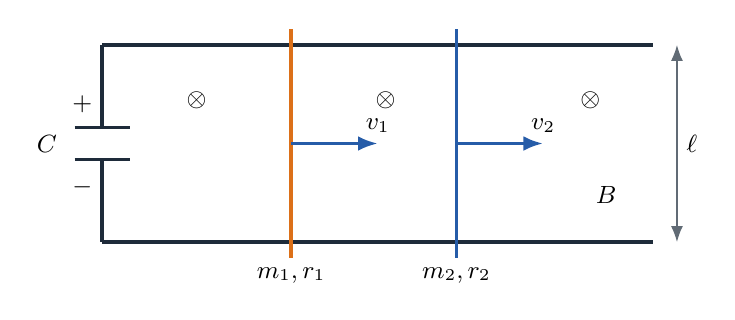
\begin{tikzpicture}[x=1cm,y=1cm,font=\small]

\draw[body] (0,0)--(7,0);\draw[body] (0,2.5)--(7,2.5);
\draw[body] (0,0)--(0,1.05);\draw[body] (-.35,1.05)--(.35,1.05);
\draw[body] (-.35,1.45)--(.35,1.45);\draw[body] (0,1.45)--(0,2.5);
\node[left] at (-.45,1.25) {$C$};\node[left] at (0,1.75) {$+$};\node[left] at (0,.7) {$-$};
\draw[body,orange] (2.4,-.2)--(2.4,2.7);\draw[body,blue] (4.5,-.2)--(4.5,2.7);
\node[below] at (2.4,-.2) {$m_1,r_1$};\node[below] at (4.5,-.2) {$m_2,r_2$};
\draw[vec] (2.4,1.25)--(3.5,1.25) node[above] {$v_1$};
\draw[vec] (4.5,1.25)--(5.6,1.25) node[above] {$v_2$};
\foreach \x in {1.2,3.6,6.2}{\node at (\x,1.8) {$\otimes$};}
\node at (6.4,.6) {$B$};\draw[dim] (7.3,0)--(7.3,2.5) node[midway,right] {$\ell$};

\end{tikzpicture}

% 14 solution-07
\begin{tikzpicture}[x=1cm,y=1cm,font=\small]

\draw[body] (0,0)--(5.8,0);\draw[body] (0,2.4)--(5.8,2.4);
\draw[body,orange] (1.5,0)--(1.5,2.4);\draw[body,blue] (4.2,0)--(4.2,2.4);
\draw[current] (1.5,.45)--(1.5,1.9) node[right] {$I_1$};
\draw[current] (4.2,.45)--(4.2,1.9) node[right] {$I_2$};
\draw[force] (1.5,1.2)--(.35,1.2) node[below] {$-bI_1$};
\draw[force] (4.2,1.2)--(3.1,1.2) node[below] {$-bI_2$};
\node[above] at (2.8,2.4) {上轨：$+$};\node[below] at (2.8,0) {下轨：$-$};
\node at (2.7,1.8) {$\otimes B$};
\node[align=left,anchor=west] at (6.4,1.5) {$r_iI_i=bv_i-V$\\[8pt] $m_i\dot v_i=-bI_i$\\[8pt] $C\dot V=I_1+I_2$};
\node[align=center] at (4,-1) {$m_1v_1+m_2v_2+bCV=\mathrm{const}$};

\end{tikzpicture}

% 15 question-08
\begin{tikzpicture}[x=1cm,y=1cm,font=\small]
\draw[body] (0,0) circle(2.2);\draw[guide] (-2.4,0)--(2.4,0);\draw[guide] (0,-2.4)--(0,2.4);
\filldraw[draw=ink,fill=blue] (1.61271,-1.49638) circle(3pt);
\filldraw[draw=ink,fill=blue] (1.98213,-0.95454) circle(3pt);
\filldraw[draw=ink,fill=blue] (2.17543,-0.32789) circle(3pt);
\filldraw[draw=ink,fill=blue] (2.17543,0.32789) circle(3pt);
\filldraw[draw=ink,fill=blue] (1.98213,0.95454) circle(3pt);
\filldraw[draw=ink,fill=blue] (1.61271,1.49638) circle(3pt);
\filldraw[draw=ink,fill=white] (1.10000,1.90526) circle(3pt);
\filldraw[draw=ink,fill=white] (0.48955,2.14484) circle(3pt);
\filldraw[draw=ink,fill=white] (-0.16441,2.19385) circle(3pt);
\filldraw[draw=ink,fill=white] (-0.80375,2.04792) circle(3pt);
\filldraw[draw=ink,fill=white] (-1.37168,1.72003) circle(3pt);
\filldraw[draw=ink,fill=white] (-1.81773,1.23930) circle(3pt);
\filldraw[draw=ink,fill=white] (-2.10226,0.64846) circle(3pt);
\filldraw[draw=ink,fill=white] (-2.20000,0.00000) circle(3pt);
\filldraw[draw=ink,fill=white] (-2.10226,-0.64846) circle(3pt);
\filldraw[draw=ink,fill=white] (-1.81773,-1.23930) circle(3pt);
\filldraw[draw=ink,fill=white] (-1.37168,-1.72003) circle(3pt);
\filldraw[draw=ink,fill=white] (-0.80375,-2.04792) circle(3pt);
\filldraw[draw=ink,fill=white] (-0.16441,-2.19385) circle(3pt);
\filldraw[draw=ink,fill=white] (0.48955,-2.14484) circle(3pt);
\filldraw[draw=ink,fill=white] (1.10000,-1.90526) circle(3pt);

\fill[red] (1.95,0) circle(3pt) node[above left] {$G$};
\node[align=left,anchor=west] at (3,.9) {实心：6条承压腿\\[8pt] 空心：15条悬空腿\\[8pt] $F_i=k\max(\delta_i,0)$\\[8pt] $\delta_i=a+b_x\cos\vartheta_i+b_y\sin\vartheta_i$};

\end{tikzpicture}

% 16 solution-08
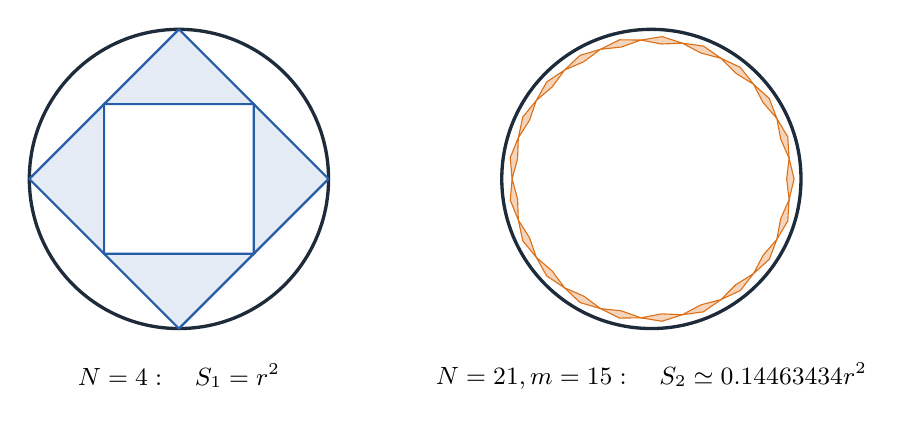
\begin{tikzpicture}[x=1cm,y=1cm,font=\small]
\draw[body] (0,0) circle(1.9);\draw[guide] (0:1.9)--(90:1.9)--(180:1.9)--(270:1.9)--cycle;
\draw[draw=blue,fill=blue!12,thick] plot coordinates {(1.900000,0.000000) (0.950000,0.950000) (0.950000,-0.950000) (1.900000,0.000000)};
\draw[draw=blue,fill=blue!12,thick] plot coordinates {(0.000000,1.900000) (-0.950000,0.950000) (0.950000,0.950000) (0.000000,1.900000)};
\draw[draw=blue,fill=blue!12,thick] plot coordinates {(-1.900000,0.000000) (-0.950000,-0.950000) (-0.950000,0.950000) (-1.900000,0.000000)};
\draw[draw=blue,fill=blue!12,thick] plot coordinates {(-0.000000,-1.900000) (0.950000,-0.950000) (-0.950000,-0.950000) (-0.000000,-1.900000)};
\node at (0,-2.5) {$N=4:\quad S_1=r^2$};
\begin{scope}[xshift=6cm]\draw[body] (0,0) circle(1.9);
\draw[draw=orange,fill=orange!30,thin] plot coordinates {(1.718298,-0.000000) (1.748908,-0.263605) (1.812619,0.000000) (1.748908,0.263605) (1.718298,-0.000000)};
\draw[draw=orange,fill=orange!30,thin] plot coordinates {(1.641959,0.506477) (1.748908,0.263605) (1.732089,0.534279) (1.593510,0.767394) (1.641959,0.506477)};
\draw[draw=orange,fill=orange!30,thin] plot coordinates {(1.419725,0.967952) (1.593510,0.767394) (1.497656,1.021084) (1.296521,1.202996) (1.419725,0.967952)};
\draw[draw=orange,fill=orange!30,thin] plot coordinates {(1.071342,1.343420) (1.296521,1.202996) (1.130149,1.417162) (0.884331,1.531707) (1.071342,1.343420)};
\draw[draw=orange,fill=orange!30,thin] plot coordinates {(0.627765,1.599519) (0.884331,1.531707) (0.662224,1.687319) (0.393564,1.724318) (0.627765,1.599519)};
\draw[draw=orange,fill=orange!30,thin] plot coordinates {(0.128409,1.713494) (0.393564,1.724318) (0.135457,1.807550) (-0.132172,1.763717) (0.128409,1.713494)};
\draw[draw=orange,fill=orange!30,thin] plot coordinates {(-0.382357,1.675217) (-0.132172,1.763717) (-0.403346,1.767173) (-0.646165,1.646401) (-0.382357,1.675217)};
\draw[draw=orange,fill=orange!30,thin] plot coordinates {(-0.859149,1.488090) (-0.646165,1.646401) (-0.906309,1.569774) (-1.102743,1.382796) (-0.859149,1.488090)};
\draw[draw=orange,fill=orange!30,thin] plot coordinates {(-1.259602,1.168740) (-1.102743,1.382796) (-1.328744,1.232894) (-1.461337,0.996323) (-1.259602,1.168740)};
\draw[draw=orange,fill=orange!30,thin] plot coordinates {(-1.548133,0.745542) (-1.461337,0.996323) (-1.633113,0.786466) (-1.690086,0.521322) (-1.548133,0.745542)};
\draw[draw=orange,fill=orange!30,thin] plot coordinates {(-1.699106,0.256099) (-1.690086,0.521322) (-1.792373,0.270157) (-1.768662,0.000000) (-1.699106,0.256099)};
\draw[draw=orange,fill=orange!30,thin] plot coordinates {(-1.699106,-0.256099) (-1.768662,-0.000000) (-1.792373,-0.270157) (-1.690086,-0.521322) (-1.699106,-0.256099)};
\draw[draw=orange,fill=orange!30,thin] plot coordinates {(-1.548133,-0.745542) (-1.690086,-0.521322) (-1.633113,-0.786466) (-1.461337,-0.996323) (-1.548133,-0.745542)};
\draw[draw=orange,fill=orange!30,thin] plot coordinates {(-1.259602,-1.168740) (-1.461337,-0.996323) (-1.328744,-1.232894) (-1.102743,-1.382796) (-1.259602,-1.168740)};
\draw[draw=orange,fill=orange!30,thin] plot coordinates {(-0.859149,-1.488090) (-1.102743,-1.382796) (-0.906309,-1.569774) (-0.646165,-1.646401) (-0.859149,-1.488090)};
\draw[draw=orange,fill=orange!30,thin] plot coordinates {(-0.382357,-1.675217) (-0.646165,-1.646401) (-0.403346,-1.767173) (-0.132172,-1.763717) (-0.382357,-1.675217)};
\draw[draw=orange,fill=orange!30,thin] plot coordinates {(0.128409,-1.713494) (-0.132172,-1.763717) (0.135457,-1.807550) (0.393564,-1.724318) (0.128409,-1.713494)};
\draw[draw=orange,fill=orange!30,thin] plot coordinates {(0.627765,-1.599519) (0.393564,-1.724318) (0.662224,-1.687319) (0.884331,-1.531707) (0.627765,-1.599519)};
\draw[draw=orange,fill=orange!30,thin] plot coordinates {(1.071342,-1.343420) (0.884331,-1.531707) (1.130149,-1.417162) (1.296521,-1.202996) (1.071342,-1.343420)};
\draw[draw=orange,fill=orange!30,thin] plot coordinates {(1.419725,-0.967952) (1.296521,-1.202996) (1.497656,-1.021084) (1.593510,-0.767394) (1.419725,-0.967952)};
\draw[draw=orange,fill=orange!30,thin] plot coordinates {(1.641959,-0.506477) (1.593510,-0.767394) (1.732089,-0.534279) (1.748908,-0.263605) (1.641959,-0.506477)};
\node at (0,-2.5) {$N=21,m=15:\quad S_2\simeq0.14463434r^2$};\end{scope}

\end{tikzpicture}
\end{document}
